\documentclass[tikz,border=4pt]{standalone}
\usepackage{helvet}
\renewcommand{\familydefault}{\sfdefault}
\definecolor{safe}{HTML}{2A9D8F}
\definecolor{fail}{HTML}{D65F5F}
\definecolor{gridline}{HTML}{FFFFFF}
\begin{document}
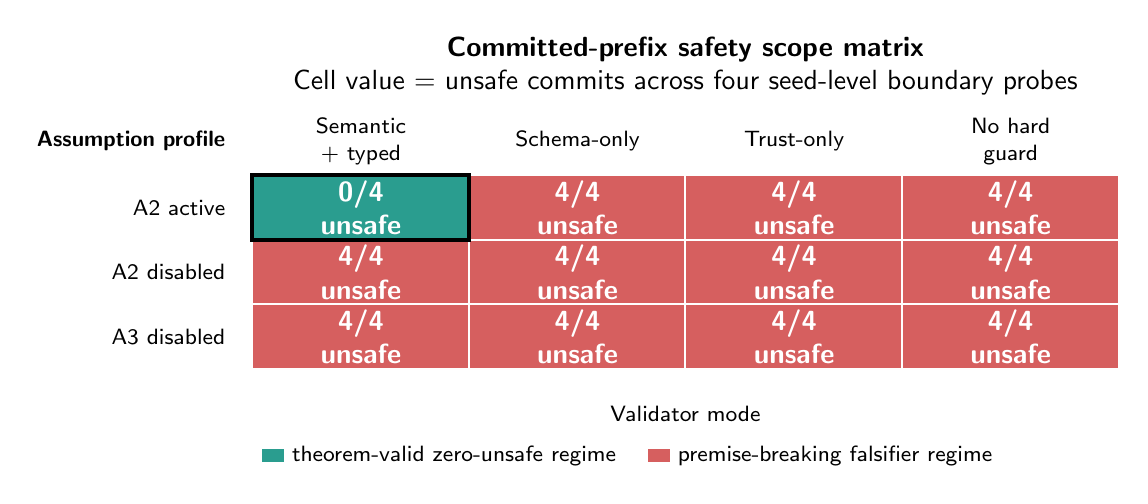
\begin{tikzpicture}[font=\sffamily\small]
\def\cellw{2.75}
\def\cellh{0.82}

\node[align=center,font=\sffamily\bfseries] at (5.5,3.65) {Committed-prefix safety scope matrix};
\node[align=center,font=\sffamily] at (5.5,3.22) {Cell value = unsafe commits across four seed-level boundary probes};

\node[anchor=east,font=\sffamily\footnotesize\bfseries] at (-0.22,2.48) {Assumption profile};
\node[align=center,font=\sffamily\footnotesize] at ({0*\cellw+1.38},2.48) {Semantic\\+ typed};
\node[align=center,font=\sffamily\footnotesize] at ({1*\cellw+1.38},2.48) {Schema-only};
\node[align=center,font=\sffamily\footnotesize] at ({2*\cellw+1.38},2.48) {Trust-only};
\node[align=center,font=\sffamily\footnotesize] at ({3*\cellw+1.38},2.48) {No hard\\guard};

\foreach \y/\lab in {
  0/{A2 active},
  1/{A2 disabled},
  2/{A3 disabled}
} {
  \node[anchor=east,font=\sffamily\footnotesize] at (-0.22,{1.64-\y*\cellh}) {\lab};
}

\newcommand{\cell}[4]{%
  \fill[#4] ({#1*\cellw},{1.23-#2*\cellh}) rectangle ++(\cellw,\cellh);
  \draw[gridline,line width=0.7pt] ({#1*\cellw},{1.23-#2*\cellh}) rectangle ++(\cellw,\cellh);
  \node[font=\sffamily\bfseries,text=white,align=center] at ({#1*\cellw+1.38},{1.64-#2*\cellh}) {#3};
}
\cell{0}{0}{0/4\\unsafe}{safe}
\cell{1}{0}{4/4\\unsafe}{fail}
\cell{2}{0}{4/4\\unsafe}{fail}
\cell{3}{0}{4/4\\unsafe}{fail}
\cell{0}{1}{4/4\\unsafe}{fail}
\cell{1}{1}{4/4\\unsafe}{fail}
\cell{2}{1}{4/4\\unsafe}{fail}
\cell{3}{1}{4/4\\unsafe}{fail}
\cell{0}{2}{4/4\\unsafe}{fail}
\cell{1}{2}{4/4\\unsafe}{fail}
\cell{2}{2}{4/4\\unsafe}{fail}
\cell{3}{2}{4/4\\unsafe}{fail}

\draw[black,line width=1.5pt] (0,1.23) rectangle ++(\cellw,\cellh);
\node[anchor=west,font=\sffamily\footnotesize] at (0,-1.52) {\tikz\fill[safe] (0,0) rectangle (0.28,0.16); theorem-valid zero-unsafe regime};
\node[anchor=west,font=\sffamily\footnotesize] at (4.9,-1.52) {\tikz\fill[fail] (0,0) rectangle (0.28,0.16); premise-breaking falsifier regime};
\node[font=\sffamily\footnotesize] at (5.5,-0.98) {Validator mode};
\end{tikzpicture}
\end{document}
